\mysection{Applications of Remote Memory Operations}
\label{section:policy}

We now discuss how hosts can use remote memory read and write operations to
analyze and control guest devices.

\myparagraph{Analysis of Guest Devices}
%
A host can analyze memory snapshots of a guest's normal world kernel
to determine its configuration and scan it for kernel malware 
(called \textit{rootkits}).

\begin{mylist}
%
\item \textit{Retrieving configuration information.} The host can determine the
kernel version by inspecting code pages, thereby also allowing it to check if
the guest has applied recommended security patches. The host can compare a hash
of each kernel code page against a whitelist, \eg~of code pages in approved
Android distributions, to ensure that the normal world is free of malicious
kernel code~\cite{patagonix:sec08,secvisor:sosp07}. Additionally, the host can
ensure that the kernel is configured to disallow well-known attack surfaces,
\eg~access to \textsf{/dev/kmem} and dynamic module loading. Finally, the host
can identify addresses at which functions of a peripheral's driver are loaded,
where they are hooked into the kernel and the addresses that store
memory-mapped peripheral settings. To do so, it can use the recursive memory
snapshot traversal technique described below. The host can use this information
to design the set of memory updates that reconfigure the device to make it
policy-compliant.
%
\item \textit{Detecting malicious data modifications.} Rootkits can
achieve malicious goals by modifying key kernel data
structures~\cite{sbcfi:ccs07,shadows:oakland07,specmon:usenix06}.  The attack
surface exposed by kernel data structures is vast.  For instance, a rootkit could
inject a device driver in kernel memory and modify kernel function pointers to
invoke methods from this driver.  Other examples of data structures that can be
misused include process lists, entropy pools used by the kernel's random number
generator, and access control
structures~\cite{shadows:oakland07,specmon:usenix06}.  
%
\end{mylist}

We now describe a generic approach, developed in prior
work~\cite{sbcfi:ccs07,gib:tdsc11,kop:ccs09,kop:sec12}, that hosts can use to
detect such malicious data modifications by analyzing the normal world's memory
snapshot. The main idea is to recursively traverse the memory snapshot and
reconstruct a view of the kernel's data structures, and use this view to reason
about the integrity of kernel data. We assume that the host has access to the
type declarations of the data structures used by the guest device's normal
world kernel, \eg~the sizes, layouts, and fields of every data structure. The
host obtains this information from trusted repositories using the kernel
version, extracted as discussed earlier.

Snapshot traversal starts from well-known entrypoints into the system's memory,
\eg~the addresses of the entities in \textsf{System.map}. When the traversal
process encounters a pointer, it fetches the memory object referenced by the
pointer and recurses until all objects have been fetched.  Having reconstructed
a view of kernel data structures, the host can then determine whether they have
been maliciously modified. For example, it could check that function pointers
in the kernel point to functions defined in the kernel's code
space~\cite{sbcfi:ccs07}. Similarly, the host can check that the kernel's data
structures satisfy invariants that typically hold in an uncompromised
kernel~\cite{gib:tdsc11}. We do not further elaborate on specific rootkit
detection policies because they are orthogonal to our focus.

A malicious or rootkit-infected OS kernel can be reliably diagnosed
\textit{only} by externally observing its code and data, \eg~using memory
snapshots as already discussed. Prior techniques that are based on
policy-enforcing normal world kernels
(\eg~\cite{asm:sec14,flaskdroid:sec13,conxsense:asiaccs14,worlddriven:ccs14,blindspot:2009,markit:upside14})
can also benefit from our approach to establish normal world kernel integrity
to hosts.

We have restricted our discussion to an analysis of the normal world's kernel
memory snapshot. In theory, it is possible for a host to also request and
analyze the normal world's user-space memory, \eg~for malicious apps that
reside in memory or on the file system. However, in practice, user-space
memory may contain sensitive information stored in apps, which guests may be
unwilling to share with hosts. For example, guests can configure their vetting
service to mark as \textsc{Unsafe} host requests to fetch user-space memory
pages (see \sectref{section:vetting}). 

To ensure user-space security, hosts can leverage the normal world kernel after
establishing that it is benign. The host can require the normal world kernel to
execute a mutually-agreed-upon anti-malware app in user-space. At check-in, the
host scans the process list in the device's kernel memory snapshot to ensure
that an anti-malware is executing. This app can check user-space memory and the
file-system for malicious activity. At check-out, it can ensure that the same
app is still executing by comparing its process identifier to the value
obtained at check-in,\footnote{The security of this scheme is based on the fact
that PIDs on UNIX systems are, for all practical purposes, unique on a given
system. For example, while they can be recycled, it requires a large counter to
wrap around.} thereby ensuring that the anti-malware app was active for the
duration of the guest's stay.

\myparagraph{Control over Guest Device Peripherals}
%
Hosts can control the availability and configuration of peripherals on guest
devices via remote memory updates to the devices. After analyzing the guest's
memory snapshot, hosts prepare a set of memory updates to control various
peripherals on guest devices. These updates can be used to simply uninstall
peripherals that may be misused violate the host's policies. Our overall
approach to controlling peripherals is to update peripheral device drivers. On
modern OSes, each peripheral has an interface within the kernel. This interface
consists of a set of function pointers that are normally set to point to the
corresponding functions within the peripheral's device driver, which
communicates with the peripheral. 

\begin{figure}[t!]
\begin{center}
\footnotesize
\begin{tabular}{|cc|}
\hline
\multicolumn{2}{|c|}{\indent\vspace{-0.3cm}}\\
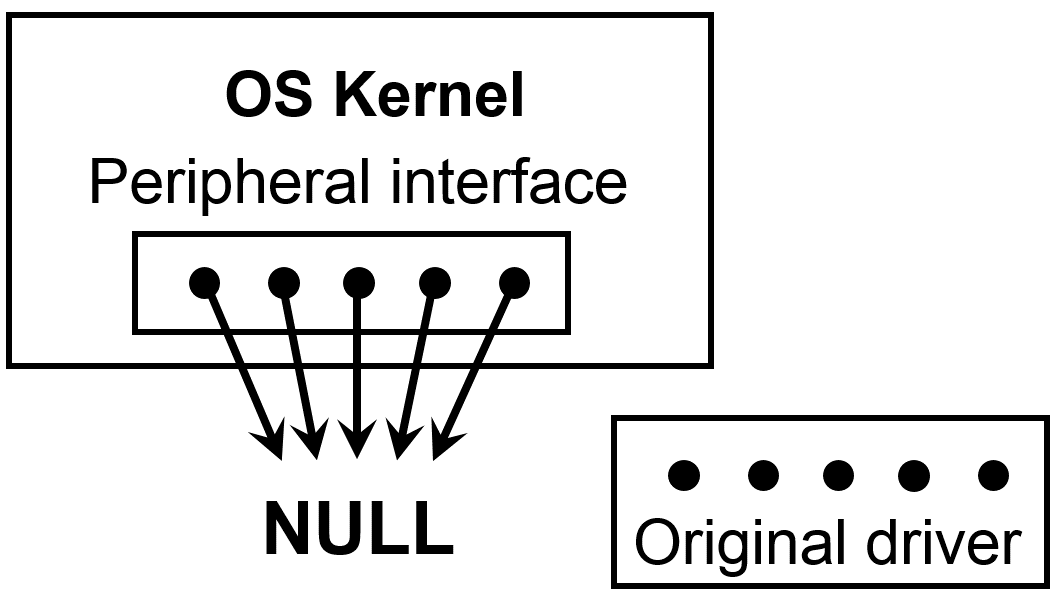
\includegraphics[keepaspectratio=true,height=0.85in]{figures/driver-null.png} & 
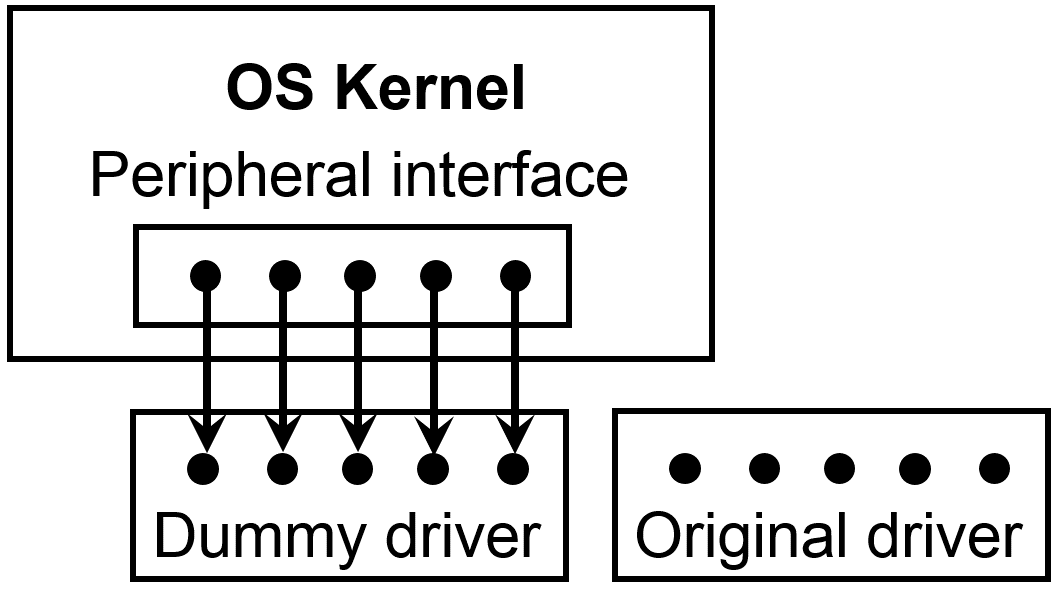
\includegraphics[keepaspectratio=true,height=0.85in]{figures/driver-dummy.png}\\
\textbf{(a)~\textsc{null}ifying the interface} &
\textbf{(b)~Installing a dummy driver}\\
%\indent\vspace{-0.9cm}
\multicolumn{2}{|p{0.47\textwidth}|}
{\small Each device driver exposes an interface and is linked to the kernel via
function pointers.  Part~(a) shows how to uninstall the peripheral by making
the kernel's device interface point to \textsc{null} bytes.  Part~(b) shows how
to uninstall the peripheral by unlinking the original driver and instead
linking a dummy driver.}\\
\hline
\end{tabular}
\end{center}
\indent\vspace{-0.5cm}
\mycaption{Uninstalling peripheral device drivers using remote write operations 
to kernel memory.}
{\label{figure:uninstall}}
\end{figure}

We adopted two broad strategies to update device drivers:  

\begin{mylist} 
%
\item \textit{Nullifying interfaces (\figref{figure:uninstall}(a)).} This
approach simply sets the function pointers in the peripheral's interface to
\textsc{null}. If the kernel checks these pointers prior to invoking the
functions, it will simply return an error code to the application saying that
the device is not installed. This approach has the advantage of only involving
simple writes to the kernel (\textsc{null} bytes to certain addresses), which
can easily be validated as safe if the guest so wishes. However, we found in
our evaluation (\sectref{section:evaluation}) that this approach can crash the
device if the kernel expects non-\textsc{null} pointers.
%
\item \textit{Dummy drivers (\figref{figure:uninstall}(b)).} In this approach,
the host writes a dummy driver for the peripheral and links it with the kernel
in place of the original driver. If the dummy driver simply return a suitable
error code rather than communicating with the peripheral, it has the effect of
uninstalling the peripheral. The error code is usually bubbled up to and
handled by user apps. Some apps may not be programmed to handle such errors, so
an alternative approach could be for the dummy driver to return synthetic
peripheral data instead of error codes~\cite{mockdroid:hotmobile10}. Dummy
drivers can also offer fine-grained peripheral control. For example, with
3G/4G, it may be undesirable to simply uninstall the modem to disable voice
messaging because it also prevents the guest from making emergency calls. The
host can avoid this by designing a dummy driver that allows calls to emergency
numbers alone, while disabling others. In this approach, the host introduces
new driver code into the guest. From the guest's perspective, this code is
untrusted and must be safety-checked by the vetting service.

\end{mylist}

